\chapter{Kajian Pustaka}

Pembelajaran mesin sudah banyak dipakai di berbagai bidang keilmuan. Mulai dari Pemrosesan Citra seperti yang di lakukan oleh Lawrence et al (2007)\cite{lawrence1997face}. Beliau menggunakan \emph{neural network} dengan tipe \emph{Convolutional Neural Network} untuk mendeteksi wajah. Van Gent et al (2007) \cite{van2007neural}, beliau menggunakan \emph{Neural Network} untuk menganalisa \emph{overtopping} gelombang pada struktur di wilayah pantai. Yau et al (2012)\cite{YAO201230}, dia mengerjakannya dengan menggunakan model \emph{Boussinesq} 1 dimensi untuk memodelkan transformasi gelombang saat melewati terumbu karang Pada bab ini akan dijelaskan model \emph{runup} gelombang pada terumbu karang menggunakan Pembelajaran Mesin.

\section{Runup Gelombang}

Runup gelombang adalah jarak vertikal maksimum dari kenaikan gelombang pada pantai atau struktur di atas \emph{SWL} \cite{sorensen2005basic}. Pada TA ini, data ovservasi ketinggian \emph{runup} gelombang diukur mulai ketinggian \emph{swl}, hingga maksimum ketinggian air di daratan. Penjelasan lebih lanjut tentang pengambilan data akan dijelaskan pada bagian \nameref{kondisiEksperimen}. Runup gelombang dapat diilustrasikan dengan gambar berikut:

\begin{figure}
    \begin{center}
        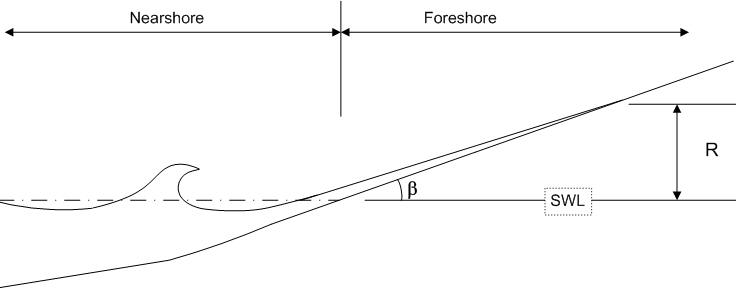
\includegraphics[scale=0.7]{./images/runup_gelombang.jpg}
    \end{center}
    \caption{Ilustrasi \emph{Runup} gelombang oleh Mike Swenson, Coastal Morphology, University of Wisconsin-Madison \cite{MikeSwenson:WaveRunup}. \emph{SWL (Sea Water Level)} adalah ketinggian Air Normal ketika tidak gelombang . Wilayah Pantai (\emph{Foreshore}), dimulai dari titik \emph{SWL} yang berpotongan dengan daratan. Wilayah lautan \emph{Nearshore}, dimulai dari titik \emph{SWL} yang berpotongan dengan air. Ketika titip potong air dengan daratan berada di atas \emph{SWL}, dinamakan \emph{runup}. Ketinggian \emph{runup} dinotasikan dengan $R$.}
\end{figure}
\FloatBarrier

\section{Pembelajaran Mesin}
    Pembelajaran mesin adalah bidang studi yang memberikan kemampuan komputer untuk belajar, tanpa harus di program secara khusus \cite{arthur_l_samuel_1959}. Mesin dikatakan belajar dari pengalaman ($E$) terhadap tugas ($T$) dan ukuran kinerja ($P$), jika kinerja pada tugas ($T$), yang di ukur berdasarkan ($P$), berkembang berdasarkan pengalaman ($E$). Dalam TA ini, akan dibuat suatu program yang dapat belajar dari data gelombang hasil observasi ($T$). Lalu dievaluasi hasilnya dengan menggunakan $MSE$ ($P$), sehingga dapat di lihat seberapa besar galatnya. Lalu diperkecil galatnya dengan metode optimasi.

\subsection{Supervised Learning}
    Sebelum data dimasukan ke dalam program, data tersebut diberikan label. Label tersebut bisa berupa \emph{input}, yakni $H$ (\emph{Significant Height} Gelombang), $T$ (\emph{Spectral Peak Periods}), dan $WL$ (\emph{Wave Length}). Dan label untuk \emph{output}. Karna pada TA kali ini, akan digunakan regresi linear. Maka tidak ada label untuk \emph{output}. Parameter \emph{input} yang berpasangan dengan \emph{output} tertentu, selanjutnya dinamakan contoh. Pembelajaran Mesin yang demikian dinamakan \emph{Supervised Learning}. \emph{Supervised Learning} Merupakan bagian dari pembelajaran mesin yang memetaan \emph{input} ke \emph{output} yang berdasar pada contoh pasangan \emph{input} dan \emph{output}\cite{AIPeterNorvig}. 

\subsection{Neural Network}
    Selanjutnya data tersebut dimasukan kedalam suatu sistem untuk belajar. Pada TA ini, sistem yang digunakan untuk pembelajaran adalah \emph{Neural Network}.
    Model \emph{neural network} sederhana di definisikan oleh McCulloch-Pitts \cite{McCulloch1943}. Dimana persamaan memiliki $M$ himpunan \emph{Input} ($I$) (\emph{input neuron}), dan satu \emph{output} ($y$), dengan $y$ merupakan bagian dari $\{0,1\}$. Atau dengan kata lain, $y$ adalah fungsi yang hanya memiliki \emph{output} $0$ dan $1$.

    \begin{equation}
        y = f(z)
    \end{equation}
    dimana
    \begin{equation}
    \label{eq:mcullochNeuralNetwork}
        z = \sum_{i=1}^N I_iW_i
    \end{equation}

    Di TA ini, \emph{output} yang akan dihasilkan tidak terbatas pada $0$ dan $1$. Sehingga di \emph{neuron output}, fungsi aktivasi yang digunakan adalah fungsi aktivasi linear. Model \emph{Neural Network}nya dapat direpresentasikan sebagai berikut:
    
    \def\layersep{5cm}

    \begin{tikzpicture}[shorten >=1pt,->,draw=black!50, node distance=\layersep]
        \tikzstyle{every pin edge}=[<-,shorten <=1pt]
        \tikzstyle{neuron}=[circle,fill=black!25,minimum size=17pt,inner sep=0pt]
        \tikzstyle{input neuron}=[neuron, fill=green!50];
        \tikzstyle{output neuron}=[neuron, fill=red!50];
        \tikzstyle{hidden neuron}=[neuron, fill=blue!50];
        \tikzstyle{annot} = [text width=4em, text centered]

        % Draw the input layer nodes
        \node[input neuron, pin=left:H] (I-H) at (0,-1) {};
        \node[input neuron, pin=left:WL] (I-T) at (0,-2) {};
        \node[input neuron, pin=left:WIND] (I-WL) at (0,-3) {};
        \node[input neuron, pin=left:T] (I-WIND) at (0,-4) {};

        % Draw the hidden layer nodes
        \path[yshift=0.0cm]{}
            node[hidden neuron] (H-1) at (\layersep,-1 cm) {};
        \path[yshift=0.0cm]{}
            node[hidden neuron] (H-2) at (\layersep,-2 cm) {};
        \path[yshift=0.0cm]{}
            node[hidden neuron] (H-3) at (\layersep,-3 cm) {};
        \path[yshift=0.0cm]{}
            node[hidden neuron] (H-4) at (\layersep,-4 cm) {};

        % Draw the output layer node
        \node[output neuron,pin={[pin edge={->}]right:Output}, right of=H-3] (O) {};

        % Connect every node in the input layer with every node in the
        % hidden layer.
        \foreach \source in {H, T, WL, WIND}
            \foreach \dest in {1,...,4}
                \path (I-\source) edge node[midway, right] {$W_{hidden}$} (H-\dest);

        % Connect every node in the hidden layer with the output layer
        \foreach \source in {1,...,4}
            \path (H-\source) edge node[midway, right] {$W_{output}$} (O);

        % Annotate the layers
        \node[annot,above of=H-1, node distance=1cm] (hl) {Hidden layer};
        \node[annot,left of=hl] {Input layer};
        \node[annot,right of=hl] {Output layer};
        \label{neuralNetworkRepresentation}
    \end{tikzpicture}

    Dimana $W$ adalah peubah yang menyatakan berat. Masing masing \emph{input} akan \emph{dot productkan} dengan $W_{input}$ \emph{hidden layer} tertentu untuk menghasilkan nilai pada \emph{hidden layer neuron} tersebut. Selanjutnya, nilai hasil aktivasi di \emph{hidden layer}, akan di \emph{dot productkan} dengan $W_{output}$. Untuk selanjutnya menjadi \emph{output}, yakni prediksi dari runup gelombang.
